\documentclass[]{article}
\usepackage{lmodern}
\usepackage{amssymb,amsmath}
\usepackage{ifxetex,ifluatex}
\usepackage{fixltx2e} % provides \textsubscript
\ifnum 0\ifxetex 1\fi\ifluatex 1\fi=0 % if pdftex
  \usepackage[T1]{fontenc}
  \usepackage[utf8]{inputenc}
\else % if luatex or xelatex
  \ifxetex
    \usepackage{mathspec}
  \else
    \usepackage{fontspec}
  \fi
  \defaultfontfeatures{Ligatures=TeX,Scale=MatchLowercase}
\fi
% use upquote if available, for straight quotes in verbatim environments
\IfFileExists{upquote.sty}{\usepackage{upquote}}{}
% use microtype if available
\IfFileExists{microtype.sty}{%
\usepackage{microtype}
\UseMicrotypeSet[protrusion]{basicmath} % disable protrusion for tt fonts
}{}
\usepackage[margin=2.54cm]{geometry}
\usepackage{hyperref}
\hypersetup{unicode=true,
            pdftitle={Assignment 4: Water Quality in Rivers},
            pdfauthor={Gabi Richichi},
            pdfborder={0 0 0},
            breaklinks=true}
\urlstyle{same}  % don't use monospace font for urls
\usepackage{color}
\usepackage{fancyvrb}
\newcommand{\VerbBar}{|}
\newcommand{\VERB}{\Verb[commandchars=\\\{\}]}
\DefineVerbatimEnvironment{Highlighting}{Verbatim}{commandchars=\\\{\}}
% Add ',fontsize=\small' for more characters per line
\usepackage{framed}
\definecolor{shadecolor}{RGB}{248,248,248}
\newenvironment{Shaded}{\begin{snugshade}}{\end{snugshade}}
\newcommand{\AlertTok}[1]{\textcolor[rgb]{0.94,0.16,0.16}{#1}}
\newcommand{\AnnotationTok}[1]{\textcolor[rgb]{0.56,0.35,0.01}{\textbf{\textit{#1}}}}
\newcommand{\AttributeTok}[1]{\textcolor[rgb]{0.77,0.63,0.00}{#1}}
\newcommand{\BaseNTok}[1]{\textcolor[rgb]{0.00,0.00,0.81}{#1}}
\newcommand{\BuiltInTok}[1]{#1}
\newcommand{\CharTok}[1]{\textcolor[rgb]{0.31,0.60,0.02}{#1}}
\newcommand{\CommentTok}[1]{\textcolor[rgb]{0.56,0.35,0.01}{\textit{#1}}}
\newcommand{\CommentVarTok}[1]{\textcolor[rgb]{0.56,0.35,0.01}{\textbf{\textit{#1}}}}
\newcommand{\ConstantTok}[1]{\textcolor[rgb]{0.00,0.00,0.00}{#1}}
\newcommand{\ControlFlowTok}[1]{\textcolor[rgb]{0.13,0.29,0.53}{\textbf{#1}}}
\newcommand{\DataTypeTok}[1]{\textcolor[rgb]{0.13,0.29,0.53}{#1}}
\newcommand{\DecValTok}[1]{\textcolor[rgb]{0.00,0.00,0.81}{#1}}
\newcommand{\DocumentationTok}[1]{\textcolor[rgb]{0.56,0.35,0.01}{\textbf{\textit{#1}}}}
\newcommand{\ErrorTok}[1]{\textcolor[rgb]{0.64,0.00,0.00}{\textbf{#1}}}
\newcommand{\ExtensionTok}[1]{#1}
\newcommand{\FloatTok}[1]{\textcolor[rgb]{0.00,0.00,0.81}{#1}}
\newcommand{\FunctionTok}[1]{\textcolor[rgb]{0.00,0.00,0.00}{#1}}
\newcommand{\ImportTok}[1]{#1}
\newcommand{\InformationTok}[1]{\textcolor[rgb]{0.56,0.35,0.01}{\textbf{\textit{#1}}}}
\newcommand{\KeywordTok}[1]{\textcolor[rgb]{0.13,0.29,0.53}{\textbf{#1}}}
\newcommand{\NormalTok}[1]{#1}
\newcommand{\OperatorTok}[1]{\textcolor[rgb]{0.81,0.36,0.00}{\textbf{#1}}}
\newcommand{\OtherTok}[1]{\textcolor[rgb]{0.56,0.35,0.01}{#1}}
\newcommand{\PreprocessorTok}[1]{\textcolor[rgb]{0.56,0.35,0.01}{\textit{#1}}}
\newcommand{\RegionMarkerTok}[1]{#1}
\newcommand{\SpecialCharTok}[1]{\textcolor[rgb]{0.00,0.00,0.00}{#1}}
\newcommand{\SpecialStringTok}[1]{\textcolor[rgb]{0.31,0.60,0.02}{#1}}
\newcommand{\StringTok}[1]{\textcolor[rgb]{0.31,0.60,0.02}{#1}}
\newcommand{\VariableTok}[1]{\textcolor[rgb]{0.00,0.00,0.00}{#1}}
\newcommand{\VerbatimStringTok}[1]{\textcolor[rgb]{0.31,0.60,0.02}{#1}}
\newcommand{\WarningTok}[1]{\textcolor[rgb]{0.56,0.35,0.01}{\textbf{\textit{#1}}}}
\usepackage{graphicx,grffile}
\makeatletter
\def\maxwidth{\ifdim\Gin@nat@width>\linewidth\linewidth\else\Gin@nat@width\fi}
\def\maxheight{\ifdim\Gin@nat@height>\textheight\textheight\else\Gin@nat@height\fi}
\makeatother
% Scale images if necessary, so that they will not overflow the page
% margins by default, and it is still possible to overwrite the defaults
% using explicit options in \includegraphics[width, height, ...]{}
\setkeys{Gin}{width=\maxwidth,height=\maxheight,keepaspectratio}
\IfFileExists{parskip.sty}{%
\usepackage{parskip}
}{% else
\setlength{\parindent}{0pt}
\setlength{\parskip}{6pt plus 2pt minus 1pt}
}
\setlength{\emergencystretch}{3em}  % prevent overfull lines
\providecommand{\tightlist}{%
  \setlength{\itemsep}{0pt}\setlength{\parskip}{0pt}}
\setcounter{secnumdepth}{0}
% Redefines (sub)paragraphs to behave more like sections
\ifx\paragraph\undefined\else
\let\oldparagraph\paragraph
\renewcommand{\paragraph}[1]{\oldparagraph{#1}\mbox{}}
\fi
\ifx\subparagraph\undefined\else
\let\oldsubparagraph\subparagraph
\renewcommand{\subparagraph}[1]{\oldsubparagraph{#1}\mbox{}}
\fi

%%% Use protect on footnotes to avoid problems with footnotes in titles
\let\rmarkdownfootnote\footnote%
\def\footnote{\protect\rmarkdownfootnote}

%%% Change title format to be more compact
\usepackage{titling}

% Create subtitle command for use in maketitle
\providecommand{\subtitle}[1]{
  \posttitle{
    \begin{center}\large#1\end{center}
    }
}

\setlength{\droptitle}{-2em}

  \title{Assignment 4: Water Quality in Rivers}
    \pretitle{\vspace{\droptitle}\centering\huge}
  \posttitle{\par}
    \author{Gabi Richichi}
    \preauthor{\centering\large\emph}
  \postauthor{\par}
    \date{}
    \predate{}\postdate{}
  

\begin{document}
\maketitle

\hypertarget{overview}{%
\subsection{OVERVIEW}\label{overview}}

This exercise accompanies the lessons in Hydrologic Data Analysis on
water quality in rivers.

\hypertarget{directions}{%
\subsection{Directions}\label{directions}}

\begin{enumerate}
\def\labelenumi{\arabic{enumi}.}
\tightlist
\item
  Change ``Student Name'' on line 3 (above) with your name.
\item
  Work through the steps, \textbf{creating code and output} that fulfill
  each instruction.
\item
  Be sure to \textbf{answer the questions} in this assignment document.
\item
  When you have completed the assignment, \textbf{Knit} the text and
  code into a single HTML file.
\item
  After Knitting, submit the completed exercise (HTML file) to the
  dropbox in Sakai. Add your last name into the file name (e.g.,
  ``A04\_Chamberlin.html'') prior to submission.
\end{enumerate}

The completed exercise is due on 25 September 2019 at 9:00 am.

\hypertarget{setup}{%
\subsection{Setup}\label{setup}}

\begin{enumerate}
\def\labelenumi{\arabic{enumi}.}
\tightlist
\item
  Verify your working directory is set to the R project file,
\item
  Load the tidyverse, dataRetrieval, cowplot, xts and dygraphs packages.
\item
  Set your ggplot theme (can be theme\_classic or something else)
\end{enumerate}

\begin{Shaded}
\begin{Highlighting}[]
\KeywordTok{getwd}\NormalTok{()}
\end{Highlighting}
\end{Shaded}

\begin{verbatim}
## [1] "/Users/gabriellerichichi/Documents/5th year @ Duke/Stats/Hydrologic_Data_Analysis/Assignments"
\end{verbatim}

\begin{Shaded}
\begin{Highlighting}[]
\KeywordTok{library}\NormalTok{(tidyverse)}
\end{Highlighting}
\end{Shaded}

\begin{verbatim}
## -- Attaching packages ----------------------------------------------------------------------------------------------- tidyverse 1.2.1 --
\end{verbatim}

\begin{verbatim}
## v ggplot2 3.2.1     v purrr   0.3.2
## v tibble  2.1.3     v dplyr   0.8.3
## v tidyr   0.8.3     v stringr 1.4.0
## v readr   1.3.1     v forcats 0.4.0
\end{verbatim}

\begin{verbatim}
## -- Conflicts -------------------------------------------------------------------------------------------------- tidyverse_conflicts() --
## x dplyr::filter() masks stats::filter()
## x dplyr::lag()    masks stats::lag()
\end{verbatim}

\begin{Shaded}
\begin{Highlighting}[]
\KeywordTok{library}\NormalTok{(dataRetrieval)}
\KeywordTok{library}\NormalTok{(cowplot)}
\end{Highlighting}
\end{Shaded}

\begin{verbatim}
## 
## ********************************************************
\end{verbatim}

\begin{verbatim}
## Note: As of version 1.0.0, cowplot does not change the
\end{verbatim}

\begin{verbatim}
##   default ggplot2 theme anymore. To recover the previous
\end{verbatim}

\begin{verbatim}
##   behavior, execute:
##   theme_set(theme_cowplot())
\end{verbatim}

\begin{verbatim}
## ********************************************************
\end{verbatim}

\begin{Shaded}
\begin{Highlighting}[]
\CommentTok{#install.packages("xts")}
\CommentTok{#install.packages("dygraphs")}
\KeywordTok{library}\NormalTok{(xts)}
\end{Highlighting}
\end{Shaded}

\begin{verbatim}
## Loading required package: zoo
\end{verbatim}

\begin{verbatim}
## 
## Attaching package: 'zoo'
\end{verbatim}

\begin{verbatim}
## The following objects are masked from 'package:base':
## 
##     as.Date, as.Date.numeric
\end{verbatim}

\begin{verbatim}
## Registered S3 method overwritten by 'xts':
##   method     from
##   as.zoo.xts zoo
\end{verbatim}

\begin{verbatim}
## 
## Attaching package: 'xts'
\end{verbatim}

\begin{verbatim}
## The following objects are masked from 'package:dplyr':
## 
##     first, last
\end{verbatim}

\begin{Shaded}
\begin{Highlighting}[]
\KeywordTok{library}\NormalTok{(dygraphs)}
\end{Highlighting}
\end{Shaded}

\hypertarget{hypoxia}{%
\subsection{Hypoxia}\label{hypoxia}}

This assignment will look at another measure of water quality - oxygen
concentration. Though not directly important for human health, oxygen in
the water column is very important for aquatic life, and so is
considered a measure of water quality. Hypoxia (low oxygen) has many
different definitions. For this assignment, we will use 2 mg/L
O\textsubscript{2} as our cut-off.

\begin{enumerate}
\def\labelenumi{\arabic{enumi}.}
\setcounter{enumi}{3}
\tightlist
\item
  Import the oxygen water quality data from New Hope Creek at Blands
  (using \texttt{readNWISqw()}, site code \texttt{02097314}, parameter
  code \texttt{00300}). Make a data frame called \texttt{O2.dat} that
  includes only the Date and O\textsubscript{2} concentration values.
  Give your data frame understandable column names.
\end{enumerate}

\begin{Shaded}
\begin{Highlighting}[]
\NormalTok{NewHopeData <-}\StringTok{ }\KeywordTok{readNWISqw}\NormalTok{(}\DataTypeTok{siteNumbers =} \StringTok{"02097314"}\NormalTok{,}
                          \DataTypeTok{parameterCd =} \StringTok{"00300"}\NormalTok{,}
                          \DataTypeTok{startDate =} \StringTok{""}\NormalTok{,}
                          \DataTypeTok{endDate =} \StringTok{""}\NormalTok{)}
\KeywordTok{names}\NormalTok{(NewHopeData)[}\DecValTok{3}\NormalTok{] <-}\StringTok{ }\KeywordTok{c}\NormalTok{(}\StringTok{"Date"}\NormalTok{)}
\KeywordTok{names}\NormalTok{(NewHopeData)[}\DecValTok{21}\NormalTok{] <-}\StringTok{ }\KeywordTok{c}\NormalTok{(}\StringTok{"O2"}\NormalTok{)}
\NormalTok{O2.dat <-}\StringTok{ }\NormalTok{NewHopeData }\OperatorTok
\StringTok{  }\KeywordTok{select}\NormalTok{(}\DecValTok{3}\NormalTok{, }\DecValTok{21}\NormalTok{)}
\end{Highlighting}
\end{Shaded}

\begin{enumerate}
\def\labelenumi{\arabic{enumi}.}
\setcounter{enumi}{4}
\tightlist
\item
  Create a ggplot of oxygen concentrations over time. Include a
  horizonal line at 2 mg/l to show the hypoxia cutoff.
\end{enumerate}

\begin{Shaded}
\begin{Highlighting}[]
\NormalTok{OxygenPlot <-}
\StringTok{  }\KeywordTok{ggplot}\NormalTok{(O2.dat, }\KeywordTok{aes}\NormalTok{(}\DataTypeTok{x =}\NormalTok{ Date, }\DataTypeTok{y =}\NormalTok{ O2)) }\OperatorTok{+}
\StringTok{  }\KeywordTok{geom_point}\NormalTok{() }\OperatorTok{+}
\StringTok{  }\KeywordTok{geom_line}\NormalTok{(}\DataTypeTok{y =} \DecValTok{2}\NormalTok{) }\OperatorTok{+}
\StringTok{  }\KeywordTok{ggtitle}\NormalTok{(}\StringTok{"Dissolved Oxygen Levels over Time"}\NormalTok{) }\OperatorTok{+}
\StringTok{  }\KeywordTok{xlab}\NormalTok{(}\StringTok{"Time"}\NormalTok{) }\OperatorTok{+}
\StringTok{  }\KeywordTok{ylab}\NormalTok{(}\KeywordTok{expression}\NormalTok{(}\StringTok{"Dissolved O"}\NormalTok{ [}\DecValTok{2}\NormalTok{]}\OperatorTok{*}\StringTok{ " (mg/L)"}\NormalTok{))}
\KeywordTok{print}\NormalTok{(OxygenPlot)}
\end{Highlighting}
\end{Shaded}

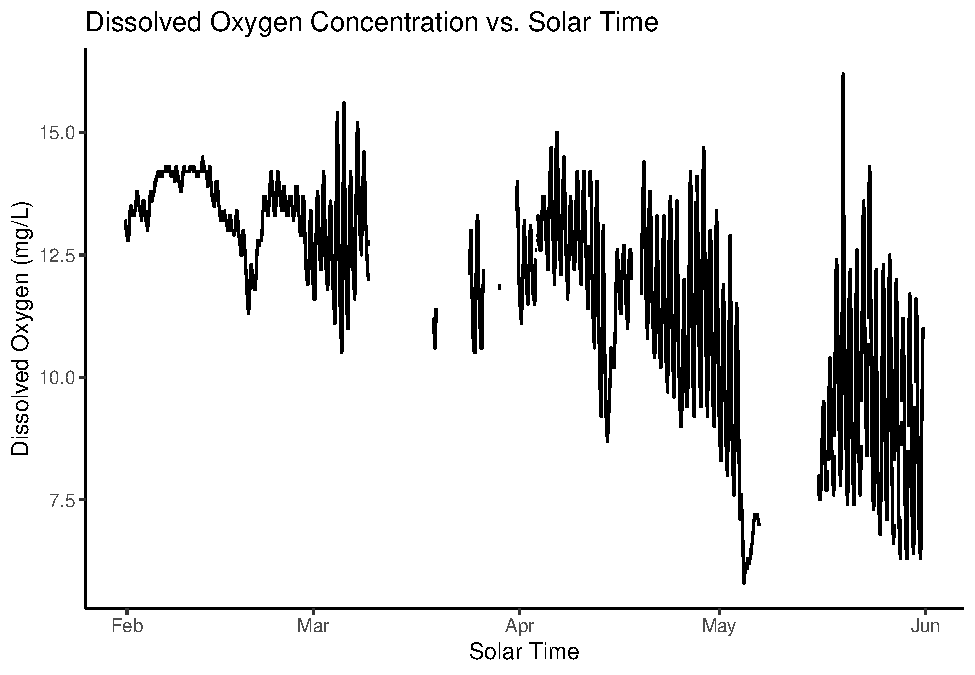
\includegraphics{A04_RiverWQ_files/figure-latex/unnamed-chunk-1-1.pdf}

\begin{enumerate}
\def\labelenumi{\arabic{enumi}.}
\setcounter{enumi}{5}
\tightlist
\item
  What do you notice about the frequency of hypoxia overtime?
\end{enumerate}

\begin{quote}
It appears that hypoxia occurred a few times in the 1980s but has not
occurred since. In the '80s, there was a wide range of dissolved oxygen
levels measured, from below 2.0 mg/L to almost 12.5 mg/L. Over time, the
dissolved oxygen levels seem to stabilize and centralize around 6 mg/L.
\end{quote}

\hypertarget{nutrients}{%
\subsection{Nutrients}\label{nutrients}}

\begin{enumerate}
\def\labelenumi{\arabic{enumi}.}
\setcounter{enumi}{6}
\tightlist
\item
  Often times hypoxia is associated with high nutrient concentrations,
  because abundant nutrients promote biomass growth which increases
  respiration and depletes oxygen concentrations in the water (remember
  how oxygen concentrations were very low in the hypolimnion from the
  Physical Properties of Lakes week). Create a new data frame, called
  \texttt{nutrients.dat} with total nitrogen (parameter code
  \texttt{00600}) and total phosphorus (parameter code \texttt{00665})
  data from the USGS. Your data frame should have 3 columns,
  \texttt{Date}, \texttt{TotalNitrogen\_mgl-N}, and
  \texttt{TotalPhosphorus\_mgl-P}.
\end{enumerate}

\begin{Shaded}
\begin{Highlighting}[]
\NormalTok{NutrientData <-}\StringTok{ }\KeywordTok{readNWISqw}\NormalTok{(}\DataTypeTok{siteNumbers =} \StringTok{"02097314"}\NormalTok{,}
                           \DataTypeTok{parameterCd =} \KeywordTok{c}\NormalTok{(}\StringTok{"00600"}\NormalTok{, }\StringTok{"00665"}\NormalTok{),}
                           \DataTypeTok{startDate =} \StringTok{""}\NormalTok{,}
                           \DataTypeTok{endDate =} \StringTok{""}\NormalTok{)}

\KeywordTok{names}\NormalTok{(NutrientData)[}\DecValTok{3}\NormalTok{] =}\StringTok{ "Date"}
\KeywordTok{names}\NormalTok{(NutrientData)[}\DecValTok{21}\NormalTok{] =}\StringTok{ "Measurements"}
\NormalTok{Nitrogen <-}\StringTok{ }\KeywordTok{filter}\NormalTok{(NutrientData, parm_cd }\OperatorTok{==}\StringTok{ "00600"}\NormalTok{)}
\NormalTok{Phosphorus <-}\StringTok{ }\KeywordTok{filter}\NormalTok{(NutrientData, parm_cd }\OperatorTok{==}\StringTok{ "00665"}\NormalTok{)}
\NormalTok{NitrogenCut <-}\StringTok{ }\NormalTok{Nitrogen }\OperatorTok
\StringTok{  }\KeywordTok{select}\NormalTok{(}\DecValTok{3}\NormalTok{, }\DecValTok{21}\NormalTok{)}
\KeywordTok{names}\NormalTok{(NitrogenCut)[}\DecValTok{2}\NormalTok{] =}\StringTok{ "TotalNitrogen_mglN"}
\NormalTok{PhosphorusCut <-}\StringTok{ }\NormalTok{Phosphorus }\OperatorTok
\StringTok{  }\KeywordTok{select}\NormalTok{(}\DecValTok{3}\NormalTok{,}\DecValTok{21}\NormalTok{)}
\KeywordTok{names}\NormalTok{(PhosphorusCut)[}\DecValTok{2}\NormalTok{] =}\StringTok{ "TotalPhosphorus_mglP"}
\NormalTok{nutrients.dat <-}\StringTok{ }\KeywordTok{left_join}\NormalTok{(NitrogenCut, PhosphorusCut, }\DataTypeTok{by =} \StringTok{"Date"}\NormalTok{)}
\end{Highlighting}
\end{Shaded}

\begin{enumerate}
\def\labelenumi{\arabic{enumi}.}
\setcounter{enumi}{7}
\tightlist
\item
  Create two ggplots stacked with cowplot that show nutrient
  concentrations over time.
\end{enumerate}

\begin{Shaded}
\begin{Highlighting}[]
\NormalTok{NPlot <-}\StringTok{ }
\StringTok{  }\KeywordTok{ggplot}\NormalTok{(nutrients.dat, }\KeywordTok{aes}\NormalTok{(}\DataTypeTok{x =}\NormalTok{ Date, }\DataTypeTok{y =}\NormalTok{ TotalNitrogen_mglN)) }\OperatorTok{+}
\StringTok{  }\KeywordTok{geom_point}\NormalTok{() }\OperatorTok{+}
\StringTok{  }\KeywordTok{xlab}\NormalTok{(}\StringTok{"Date"}\NormalTok{) }\OperatorTok{+}
\StringTok{  }\KeywordTok{ylab}\NormalTok{(}\StringTok{"Total Nitrogen (mg/L)"}\NormalTok{)}
\KeywordTok{print}\NormalTok{(NPlot)}
\end{Highlighting}
\end{Shaded}

\includegraphics{A04_RiverWQ_files/figure-latex/nutrient.plots}-1.pdf)

\begin{Shaded}
\begin{Highlighting}[]
\NormalTok{PPlot <-}
\StringTok{  }\KeywordTok{ggplot}\NormalTok{(nutrients.dat, }\KeywordTok{aes}\NormalTok{(}\DataTypeTok{x =}\NormalTok{ Date, }\DataTypeTok{y =}\NormalTok{ TotalPhosphorus_mglP)) }\OperatorTok{+}
\StringTok{  }\KeywordTok{geom_point}\NormalTok{() }\OperatorTok{+}
\StringTok{  }\KeywordTok{xlab}\NormalTok{(}\StringTok{"Date"}\NormalTok{) }\OperatorTok{+}
\StringTok{  }\KeywordTok{ylab}\NormalTok{(}\StringTok{"Total Phosphorus (mg/L)"}\NormalTok{)}
\KeywordTok{print}\NormalTok{(PPlot)}
\end{Highlighting}
\end{Shaded}

\includegraphics{A04_RiverWQ_files/figure-latex/nutrient.plots}-2.pdf)

\begin{Shaded}
\begin{Highlighting}[]
\NormalTok{CombinedNP <-}
\StringTok{  }\KeywordTok{plot_grid}\NormalTok{(NPlot, PPlot, }\DataTypeTok{ncol =} \DecValTok{1}\NormalTok{)}
\KeywordTok{print}\NormalTok{(CombinedNP)}
\end{Highlighting}
\end{Shaded}

\includegraphics{A04_RiverWQ_files/figure-latex/nutrient.plots}-3.pdf)

\begin{enumerate}
\def\labelenumi{\arabic{enumi}.}
\setcounter{enumi}{8}
\tightlist
\item
  What do these plots tell you about nutrient concentrations over time?
  How might this relate to your previous plot of hypoxia events?
\end{enumerate}

\begin{quote}
Nutrient concentrations were very high in the 1980s. One data point for
Total Nitrogen reached about 30 mg/L, and one data point for Total
Phosphorus reached about 5 mg/L. After the mid-1980s, total nutrient
levels stabilized at below 5 mg/L for nitrogen and below 1 mg/L for
phosphorus. Nutrient levels are correlated with dissolved oxygen levels.
As nutrient levels increase, phytoplankton are able to utilize those
additional nutrients to synthesize food, and they subsequently expel
oxygen. As a result, oxygen levels increase, the phytoplankton respire
the oxygen at night, some phytoplankton cells die and are decomposed,
and DO levels decrease. The river is then at risk of hypoxia. Therefore,
when nutrients levels increased in the 1980s, it makes sense that oxygen
levels both increased and decreased, even to the point of hypoxia.
\end{quote}

\hypertarget{discharge-and-temperature}{%
\subsection{Discharge and Temperature}\label{discharge-and-temperature}}

\begin{enumerate}
\def\labelenumi{\arabic{enumi}.}
\setcounter{enumi}{9}
\tightlist
\item
  Turbulent flow in rivers mixes oxygen into the water column. As
  discharge decreases, water moves slower, and oxygen diffuses slower
  into the water from the atmosphere. Download and reformat the daily
  discharge data for New Hope Creek (function \texttt{readNWISdv()},
  site \texttt{02097314}, parameter \texttt{00060}).
\end{enumerate}

\begin{Shaded}
\begin{Highlighting}[]
\NormalTok{NewHopeDischarge <-}\StringTok{ }\KeywordTok{readNWISdv}\NormalTok{(}\DataTypeTok{siteNumbers =} \StringTok{"02097314"}\NormalTok{,}
                               \DataTypeTok{parameterCd =} \StringTok{"00060"}\NormalTok{)}
\KeywordTok{names}\NormalTok{(NewHopeDischarge)[}\DecValTok{4}\OperatorTok{:}\DecValTok{5}\NormalTok{] =}\StringTok{ }\KeywordTok{c}\NormalTok{(}\StringTok{"Discharge"}\NormalTok{, }\StringTok{"Approval.Code"}\NormalTok{)}
\end{Highlighting}
\end{Shaded}

\begin{enumerate}
\def\labelenumi{\arabic{enumi}.}
\setcounter{enumi}{10}
\tightlist
\item
  Create a dygraph of discharge and oxygen concentrations. You should
  have discharge on the y axis and oxygen concentration on the y2 axis.
  Set your y-axes limits so that they don't change as you zoom in and
  out. (hint: use \texttt{dyAxis(...,\ valueRange\ =\ c(0,\ 6500))} for
  discharge \& \texttt{dyAxis(...,\ valueRange\ =\ c(0,\ 13))} for
  oxygen).
\end{enumerate}

\begin{Shaded}
\begin{Highlighting}[]
\CommentTok{#Discharge <- NewHopeDischarge$Discharge}
\CommentTok{#OxygenConc <- NewHopeData$O2}
\CommentTok{#NewPlot <-}
\CommentTok{#  dygraph(NewHopeDischarge, NewHopeData, aes(x = Date, y1 = Discharge, y2 = O2)) +}
\CommentTok{#  dyAxis(valueRange = c(0, 6500)) +}
\CommentTok{#  dyAxis(valueRange = c(0, 13))}
\CommentTok{#print(NewPlot)}
\end{Highlighting}
\end{Shaded}

\begin{enumerate}
\def\labelenumi{\arabic{enumi}.}
\setcounter{enumi}{11}
\tightlist
\item
  Do hypoxic events happen in the wet or the dry season? How many days
  after storm events (of at least 100 cfs) do they occur?
\end{enumerate}

\begin{quote}
Hypoxic events occur in the wet season, when runoff transports nutrients
from agricultural fields into rivers and other bodies of water.
\end{quote}

\begin{enumerate}
\def\labelenumi{\arabic{enumi}.}
\setcounter{enumi}{12}
\tightlist
\item
  Temperature also impacts the solubility of oxygen in water. More
  oxygen can dissolve when temperatures are \emph{lower}. How would you
  analyze the effects of temperature on dissolved oxygen concentrations?
  What data would you need? How would you separate the effects of
  temperature from the effects of flow?
\end{enumerate}

\begin{quote}
In order to analyze the effects of temeprature on dissolved oxygen
concentrations, you would need to measure both the temeperature and the
dissolved oxygen concentrations of a river over time. You would then
plot the data and see if there is a correlation. You would separate the
effects of temperature from the effects of flow by measuring the flow at
various points in the river and plotting it against the temperature and
dissolved oxygen data.
\end{quote}

\begin{enumerate}
\def\labelenumi{\arabic{enumi}.}
\setcounter{enumi}{13}
\tightlist
\item
  What do you think is the biggest driver of hypoxia in New Hope Creek?
  What data do you use to support your conclusion?
\end{enumerate}

\begin{quote}
The biggest driver of hypoxia in New Hope Creek appears to be nutrient
concentration, since nutrient concentration and dissolved oxygen levels
are highly correlated over a long time frame, from the 1980s until
present day.
\end{quote}

\hypertarget{reflection}{%
\subsection{Reflection}\label{reflection}}

\begin{enumerate}
\def\labelenumi{\arabic{enumi}.}
\setcounter{enumi}{14}
\tightlist
\item
  What are 2-3 conclusions or summary points about river water quality
  you learned through your analysis?
\end{enumerate}

\begin{quote}
I have learned: 1) That nutrient levels correlate with dissolved oxygen
levels. 2) That hypoxia is the absence of oxygen, and that hypoxia is
caused by a boom in production followed by algal respiration and death.
3) That temperature can also affect dissolved oxygen levels, which could
be compounded by flow.
\end{quote}

\begin{enumerate}
\def\labelenumi{\arabic{enumi}.}
\setcounter{enumi}{15}
\tightlist
\item
  What data, visualizations, and/or models supported your conclusions
  from 15?
\end{enumerate}

\begin{quote}
The ggplots of Dissolved Oxygen, Nitrogen, and Phosphorous over time
were very convincing. There is a clear correlation.
\end{quote}

\begin{enumerate}
\def\labelenumi{\arabic{enumi}.}
\setcounter{enumi}{16}
\tightlist
\item
  Did hands-on data analysis impact your learning about water quality
  relative to a theory-based lesson? If so, how?
\end{enumerate}

\begin{quote}
Yes, I believe that actually creating the graphs was more effortful than
just viewing graphs that were already created in a textbook, for
example. I will remember the data trends more since I put in more
effort.
\end{quote}

\begin{enumerate}
\def\labelenumi{\arabic{enumi}.}
\setcounter{enumi}{17}
\tightlist
\item
  How did the real-world data compare with your expectations from
  theory?
\end{enumerate}

\begin{quote}
The real-world data aligned with my expectations in terms of the fact
that increased nutrient concentrations are correlated with hypoxic
events. However, I would have assumed that hypoxia is worse now, in
present day, than it was in the 1980s, just because some environmental
problems such as climate change have been exacerbated recently.
\end{quote}


\end{document}

tinytex::parse_packages()
